\section{Введение}
\label{sec:Chapter0} \index{Chapter0}

\hspace{0.6cm}Большие нейронные модели NLP, в первую очередь BERT/GPT-подобные модели \cite{general1}, \cite{general2}, получили широкое распространение как в исследованиях, так и в промышленности, ввиду установленной зависимости между размером модели и ее результативностью при  решении задач. Однако как следствие, подобные модели обычно рассматриваются в виде некоторого \textbf{"чёрного ящика"}. Поэтому растёт озабоченность работой и надёжностью данных моделей, так как подобные системы часто принимают участие при принятии решений в различных сферах, где цена ошибки очень высока.

Зачастую невозможно учесть все виды отказов и проблем, которые могут возникнуть при эксплуатации данных моделей, поэтому оценка качества также должна проводиться с помощью модельных пояснений. Предоставление этих пояснений часто является основной мотивацией для понятия \textbf{“интерпретируемости”} моделей машинного и глубокого обучения. То есть, когда модели выдают неверный результат или их поведения начинает отклоняться от стандартного и первоначального задуманного, возникает необходимость в объяснениях, почему модель приняла то или иное решение на основе полученных входных данных. На сегодняшний день существует немало способов, которые могут позволить изучить поведение модели. Таковыми могут быть \textbf{состязательные примеры}.

\textbf{Состязательные примеры} - это специально подобранные входные данные, которые могут ввести в заблуждение или заставить ошибиться модель. В области обработки естественного языка (NLP) состязательные примеры могут быть созданы различными методами, такими как перефразирование текста, вставка опечаток, добавление отвлекающих элементов или замена слов синонимами. Цель состязательных примеров в NLP - проверить и улучшить устойчивость и надёжность моделей глубокого обучения. В данной работе в дальнейшем будут рассмотрены уже существующие на сегодняшний момент методы генерации состязательных примеров для текстов.

Также наряду с понятием состязательных примеров вводится понятие \textbf{состязательная устойчивость} — это мера восприимчивости модели к состязательным примерам. Её часто измеряют, используя процент попыток, которые приводят к успешным атакам. \textbf{Состязательным возмущением} же обычно называют то, насколько сильно состязательный пример отличается от исходного.

Хотя атаки в NLP не могут найти такое состязательное возмущение, которое буквально неотличимо от исходного ввода, так как данные являются дискретными, а не непрерывными, они могут найти возмущение, которое очень похоже. Состязательные атаки NLP можно разделить на две группы, основанные на их понятиях «сходства».

\begin{figure}[h]
    \centering
    \begin{adjustbox}{max width=\linewidth}
        %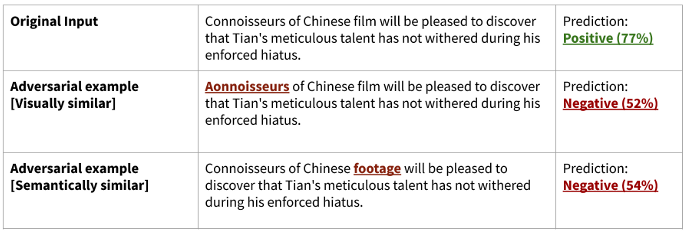
\includegraphics[width=16.6cm, height=5.5cm]{pictures/texts_similarity.png}
        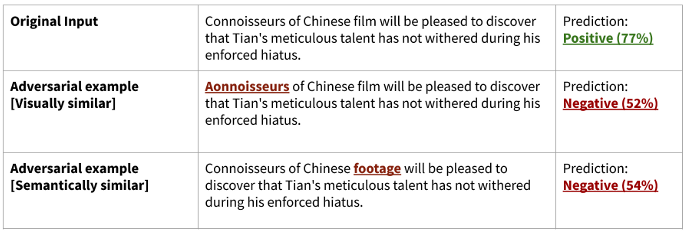
\includegraphics{pictures/texts_similarity.png}
    \end{adjustbox}
    \caption{Иллюстрация различных видов схожести текстов}
    \label{fig:texts_similarity}
\end{figure}

\noindent\hspace{0.6cm}\textbf{Визуальное сходство}: при котором исходный и состязательный текст едва отличимы друг от друга при зрительном обращении, но при этом изначальный смысл может быть искажен. На Рис. 1 видно, что слово \textcolor[RGB]{0,128,0}{Connoisseurs} было подменено похожим на него с точки зрения написания словом \textcolor[RGB]{128,0,0}{Aonnoisseurs}. То есть смысл текста был искажен, но заметить данную опечатку можно не сразу. \textbf{Семантическое сходство}: при котором два исходный и состязательный текст имеют схожий смысл, но при этом имеет явные отличия при зрительном обращении. На Рис. 1 видно, что слово \textcolor[RGB]{0,128,0}{film} было заменено синонимом \textcolor[RGB]{128,0,0}{footage}. То есть смысл текста был сохранен, однако видно, что сам текст был слегка видоизменен.

\noindent\hspace{0.6cm}Однако вопрос оптимизации порождения состязательных примеров является не менее важным, чем их генерации. В дальнейшем будет показано, что сами по себе методы генерации не могут должным образом достичь наилучшего эффекта. В данной работе будут рассмотрены различные подходы, которые позволяют выделять слова в тексте, наибольшим образом влияющие на итоговое предсказание. Данные методы опираются на выходы модели или внутренную (латентную) структуру данных в ходе её работы. Тем самым за счет атаки наиболее важных слов в тексте для модели в совокупности с существующими методами порождения можно повысить эффективность состязательных примеров.
